\subsection{Simple Polygons}
\label{sec:warm-up}

To get a sense of the types of problems we will encounter,
we begin by deriving a formula for the area
of a simple polygon on the sphere in terms of the 
interior angles.
\begin{theorem}\label{thm:triangle}
In the plane, the sum of the interior angles of a triangle is $\pi$.
\end{theorem}
\begin{proof}
Draw a line parallel to one edge through the opposite vertex.
By alternating interior angles in the plane, the sum of the angles
in the triangle equal  a straight line.
See \figref{angles} for an illustration. 



\begin{figure}[htb]
\centering
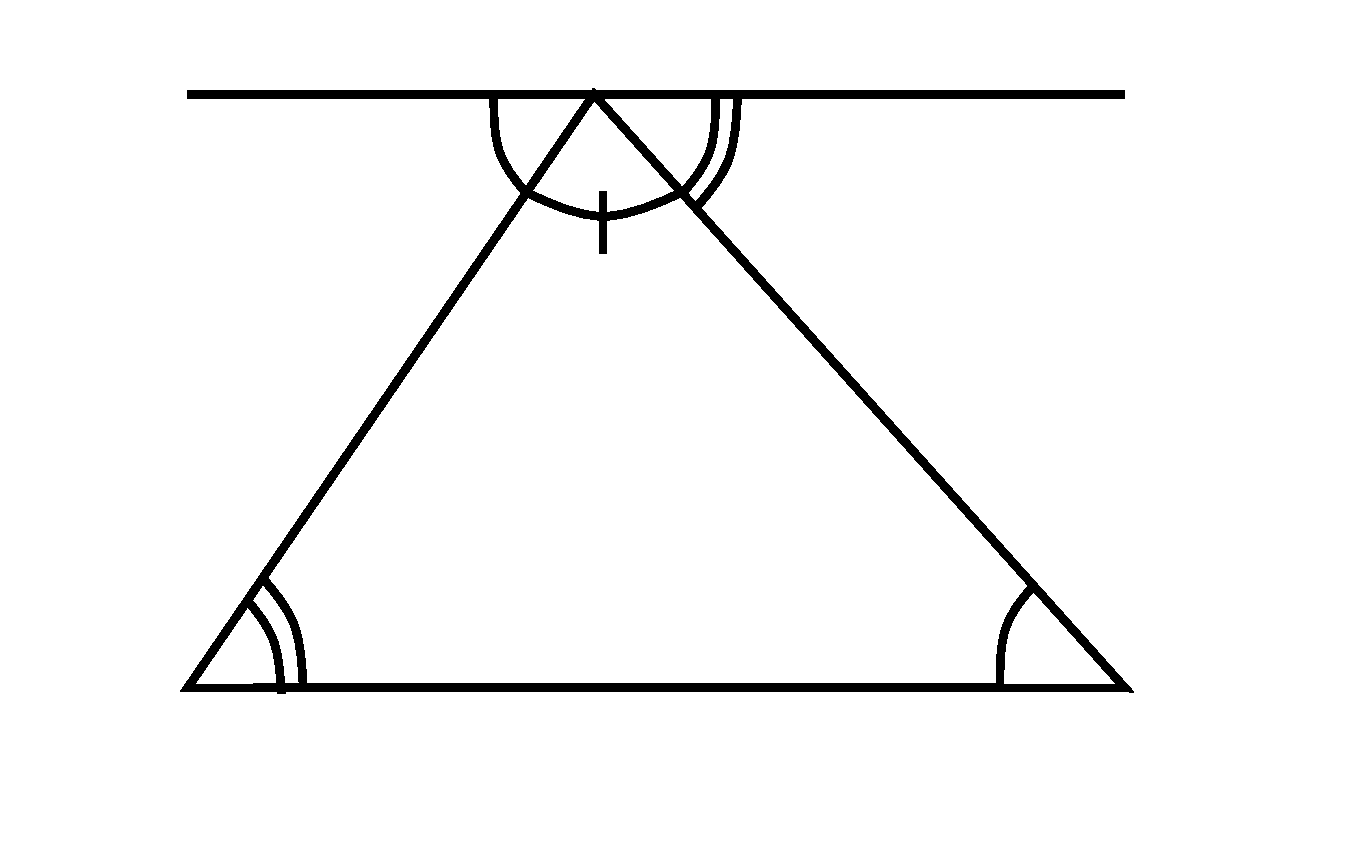
\includegraphics[width=.3\textwidth]{background/interior-angles-triangle}
\caption{A proof that, in the plane, the sum of the angles of a triangle is $\pi$.}
\label{fig:angles}
\end{figure}

\end{proof}



Consider any simple polygon in the plane $P$ with $n$ vertices. 
Then $P$ can be triangulated with $n-2$ triangles \cite{orourke_computational_1994}.
Thus, when we traverse $P$ we go around $n-2$ triangles each contributing
$\pi$.
We have
\begin{corollary}\label{cor:angles}
In the plane, any simple polygon $P$ with $n$ vertices,
the sum of the interior angles of $P$ is $(n-2)\pi$.

\end{corollary}

Now consider a triangle on the two dimensional sphere as in \figref{sphere-triangle}.

\begin{figure}[htb]
\centering
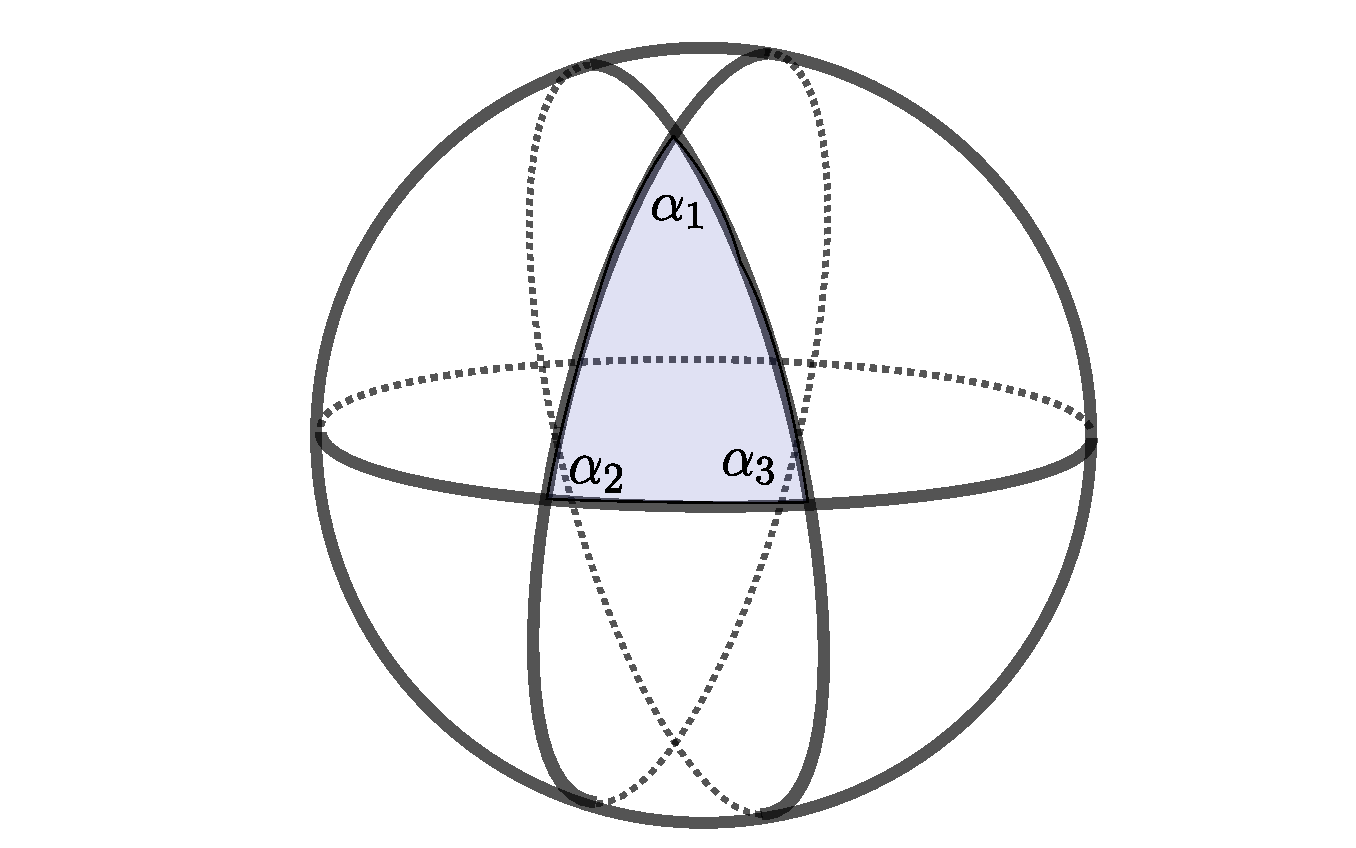
\includegraphics[width=.5\textwidth]{background/sphere-triangle}
\caption{A triangle on the sphere.}
\label{fig:sphere-triangle}
\end{figure}


\begin{figure}[htb]
\centering
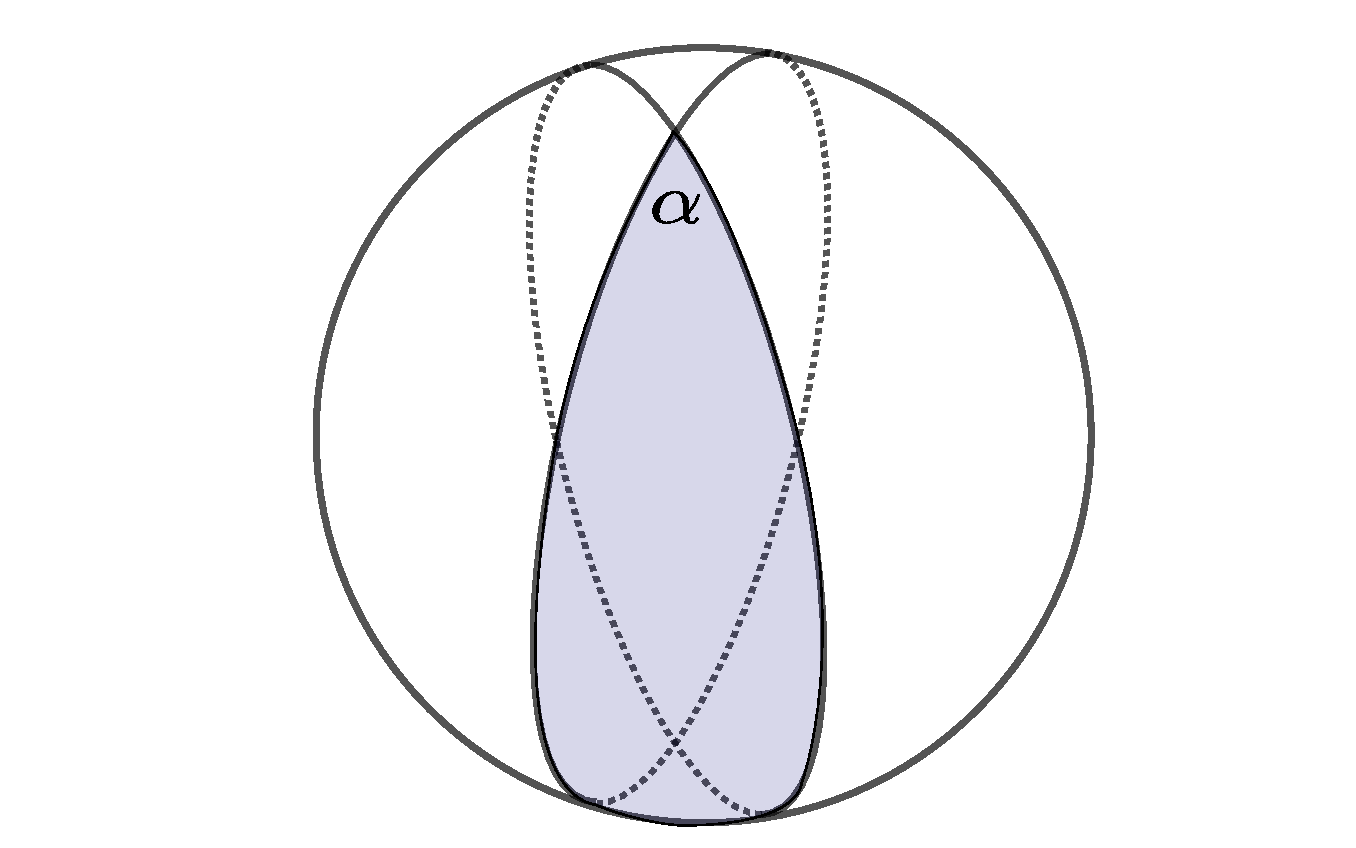
\includegraphics[width=.4\textwidth]{background/lune}
\caption{A lune with angle $\alpha$.}
\label{fig:lune}
\end{figure}